\chapter{Proposed Method and Implementation}
\label{ch:method}

This chapter describes the structure of the system, how the data were built, and
the design of the experiments. The order is: first the early attempt and the lesson
learned from it; then the dataset construction pipeline; then the architecture of
the delivered cascade, the interruption detection module and the full-duplex
transport layer; then the design of the direct-track experiments; and finally the
evidence-first way of working that frames all evaluations of the next chapter.

\section{Early Attempt and Revision of the Architecture}
\label{sec:early-attempt}

The project's first implementation was built on the LLaMA-Omni2 architecture: a
frozen Whisper speech encoder, a trainable projector, the
Qwen2.5-0.5B~\cite{qwen2025qwen25} language model with a LoRA adapter, and separate
heads for recognition and for generating speech tokens. This artifact was trained
and its loss decreased.

An internal code audit, before any result was reported, revealed three fundamental
defects that must be recorded for the methodological honesty of this report:

\begin{itemize}
\item The language model did not take part in the forward pass; what was trained was
      therefore an audio mapping network, not a dialogue-oriented language model.
\item The recognition target used per-process randomized hashes, so the training
      labels were unstable across runs.
\item The speech generation target was ``reconstruction of the same input
      utterance'', not the generation of a conversational reply; and to hear the
      output, an external speech engine bypassed the path of the learned artifact.
\end{itemize}

The conclusion of this audit was explicit: that artifact was not a speech-to-speech
model and could not be reported as one. This experience led to two decisive
decisions. First, serving was moved entirely to a cascade of real, testable
components. Second, for the direct track only a model with an ``official trainer''
was accepted, so that the training objective and data pipeline are set by the
model's authors rather than rewritten locally. These two decisions shaped the final
project.

\section{Construction of the Persian Conversational Dataset}
\label{sec:data}

\subsection{Source and Strategy}

Since no public Persian corpus with interruption labels was available
(Section~\ref{sec:persian-resources}), the dataset of this project was derived from an
internal archive of Persian spoken content. The archive contains long conversational
programmes from four channels with different styles. Internal research use of these
resources was recorded with the supervisor's approval; this approval is not a licence
to redistribute the raw audio or captions, and no restricted data were placed in the
code repository.

A methodological point corrected midway is worth recording. In the first design, the
text label of each segment was produced by re-running the speech recognition service.
But that service had itself been tuned earlier on the captions of these same
channels. Using it as the ``teacher'' therefore created a ``circular loop'' and fixed
its own systematic errors as reference labels. Once this problem was identified, the
text labels were switched to the original source captions, and the recognition
service was kept only as a runtime component and a measurement tool.

\subsection{Pipeline Stages}

Figure~\ref{fig:pipeline} shows the stages of the data pipeline.

\begin{figure}[ht]
\centering
\begin{tikzpicture}[
  node distance=3.6mm,
  stage/.style={draw,rounded corners=2pt,align=center,font=\scriptsize,
                text width=27mm,minimum height=9.5mm,inner sep=2pt},
  outbox/.style={stage,fill=black!5},
  ar/.style={-{Latex[length=1.6mm]},thin}
]
\node[stage] (inv)  {channel inventory\\775.887 h captions};
\node[stage,below=of inv]  (sel)  {weighted episode\\selection};
\node[stage,below=of sel]  (win)  {15-minute window\\reconstruction};
\node[stage,below=of win]  (dia)  {speaker\\diarization};
\node[stage,below=of dia]  (noi)  {noise-condition\\labelling};

\node[stage,right=14mm of inv]  (pair) {non-reused\\response pairs};
\node[stage,below=of pair]      (grp)  {session-group\\split};
\node[stage,below=of grp]       (pip)  {Piper assistant\\re-synthesis};
\node[stage,below=of pip]       (exp)  {stereo export\\+ text alignment};
\node[outbox,below=of exp]         (aud)  {integrity audit\\108.584 h};

\draw[ar] (inv) -- (sel);
\draw[ar] (sel) -- (win);
\draw[ar] (win) -- (dia);
\draw[ar] (dia) -- (noi);
\draw[ar] (noi.east) -- ++(0.7,0) |- (pair.west);
\draw[ar] (pair) -- (grp);
\draw[ar] (grp) -- (pip);
\draw[ar] (pip) -- (exp);
\draw[ar] (exp) -- (aud);
\end{tikzpicture}
\caption{Stages of the Persian conversational dataset pipeline. Each stage is a
         separate command with an auditable output.}
\label{fig:pipeline}
\end{figure}

\paragraph{Inventory and selection.} The measurable inventory of the archive was
775.887 hours of captions in 1,442 long programmes. A weighted, \emph{deterministic}
selection was run on this inventory, aimed at balancing the channels and avoiding the
dominance of one speaking style. The output of this stage is 309 programmes and 1,129
windows with a total of 219.946 candidate hours.

\paragraph{Window reconstruction.} The source programmes were stored as small chunks.
To preserve the structure of the conversation, the chunks were reconstructed into
continuous 15-minute windows. This length is long enough to contain several complete
dialogue turns.

\paragraph{Speaker diarization.} Each window was given to the diarization service,
which returns the time boundaries and speaker identity of each speech segment as well
as the overlap segments. The total of automatically classified multi-speaker segments
is 207.154 hours.

\paragraph{Noise-condition labelling.} For each segment, a noise-condition label
based on an estimated signal-to-noise ratio was added, so that the effect of acoustic
conditions can be separated in later analyses.

\paragraph{Why the MFA forced aligner was not used.} The proposal suggests the
Montreal Forced Aligner~\cite{mcauliffe2017mfa} for marking turns and overlaps. Forced
alignment places known text within the audio of \emph{one speaker}, but it does not say
which speaker talks when or where two voices overlap; the turn boundaries and overlap
segments therefore came from speaker diarization, and the text of each turn from the
caption timing. Where word-by-word timing was needed --- the assistant speech in the
seventh version of the direct track (Section~\ref{sec:moshi-v7}) --- no statistical
aligner was needed: that speech had been generated by Piper itself, and the time of
each phoneme was taken from the same synthesizer's phoneme-to-sample alignment in an
identical re-synthesis.

\subsection{Response-Pair Extraction and Interaction Labels}
\label{sec:pairs}

From the diarized segments, ``user speech and the next speaker's response'' pairs are
extracted. First, consecutive segments of one speaker less than half a second apart
are merged into a complete turn. Then a pair is built for every two consecutive turns
of two different speakers.

An important constraint of this stage is ``no reuse'': each segment of the source
audio appears in only one pair. This constraint is needed because reuse would
artificially inflate the number of reported hours and would act as data repetition in
training.

For each pair an automatic interaction label is also computed. If the second turn
starts before the first turn ends, there is overlap. In that case, if the second turn
is short and ends before the first turn ends, the label is ``backchannel'', and
otherwise ``interruption''. If the overlap cannot be attributed to a speaker, the
label ``unattributed overlap'' is recorded.

The output of this stage is 6,754 pairs with 123.796 hours of source audio. In
addition, 770 conservative interaction-event candidates (717 interruption-like and 53
backchannel-like) were recovered from the speaker boundaries.

\claim{These labels are entirely \emph{automatic}. The forty-row listening review of
the data and the twenty-four-row review of interaction events were not run, under a
documented time waiver. Therefore no row is reported as ``human-verified'' anywhere in
this report, and the number of human-verified labels is zero.}

\subsection{Group Splits and Re-Synthesis of the Response Voice}

Training, validation and test splits were made by source session identifier with
deterministic hashing (Section~\ref{sec:group-split}). The result is 6,419 training
pairs, 131 validation pairs and 204 test pairs, and the automatic audit confirms zero
group leakage.

For the direct track, the ``assistant'' channel must not carry the voices of the many
source speakers, because the model has to learn one stable target voice. The text of
the response turn was therefore re-synthesized with the Persian speech engine and one
fixed, \emph{deterministic} voice. This is standard practice in training
speech-to-speech models. The final output is one stereo audio file per pair, with
channel zero the assistant's speech and channel one the user's speech, together with
an adjacent text alignment file.

The total exported stereo audio is a measured 108.584 hours, which lies within the
100--200 hours targeted by requirement R4. Figure~\ref{fig:corpus} shows the gradual
reduction in volume from the raw inventory to the audited export.

\begin{figure}[ht]
\centering
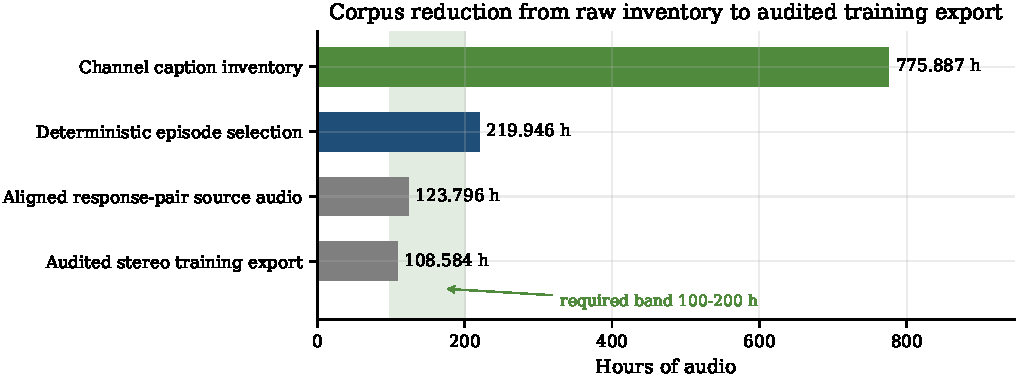
\includegraphics[width=0.95\textwidth]{figs/corpus_funnel.pdf}
\caption{Gradual reduction of the amount of audio from the channels' caption inventory
         to the audited stereo training export. The light band shows the 100--200
         hours targeted by the project definition.}
\label{fig:corpus}
\end{figure}

\section{Architecture of the Streaming Cascade}
\label{sec:cascade}

The delivered system is a streaming cascade on top of which full-duplex control is
built (Figure~\ref{fig:arch}). The first version of this chain worked with a
``push-to-talk'' button, built the whole reply before playback and ran all three
stages one after another inside one process; our estimate of its latency from end of
speech to first audio was about 2.2 seconds (median). In the final version each stage
overlaps with the next: the end of speech is detected automatically, reply generation
starts before the end of speech is confirmed, tokens arrive as a stream, and each
clause of the sentence is synthesized and played as soon as it is complete.

\begin{figure}[ht]
\centering
\scalebox{0.92}{%
\begin{tikzpicture}[
  box/.style={draw,rounded corners=2pt,align=center,font=\scriptsize,
              minimum height=9mm,inner sep=3pt,text width=23mm},
  client/.style={box,fill=black!5},
  lbl/.style={font=\scriptsize,inner sep=1.5pt,fill=white},
  ar/.style={-{Latex[length=1.8mm]},thin},
  dashar/.style={ar,dashed}
]
\node[client] (mic) at (0,0) {browser mic\\20 ms PCM16 frames\\+ playback level};
\node[box] (vad)  at (3.2,-2.3) {Silero VAD endpointer\\speculative 96 ms\\confirm 256 ms};
\node[box] (asr)  at (6.4,-2.3) {NeMo v4 CTC\\ASR};
\node[box] (llm)  at (9.6,-2.3) {Qwen3-4B (vLLM)\\streamed, Persian-only};
\node[box] (tts)  at (12.8,-2.3) {clause chunker\\+ Mana Piper (CPU)};
\node[box] (dtd)  at (3.2,0) {double-talk detector\\+ Silero: \emph{duck}};
\node[box] (lex)  at (6.4,0) {lexical confirm\\(ASR, echo words,\\listener tokens)};
\node[client] (spk) at (12.8,0) {browser playback\\queue: duck / stop};
\draw[ar] (mic) |- (vad.west) node[lbl,pos=0.75] {listening};
\draw[ar] (vad) -- (asr);
\draw[ar] (asr) -- (llm);
\draw[ar] (llm) -- (tts);
\draw[ar] (tts) -- (spk) node[lbl,midway] {per clause};
\draw[ar] (mic) -- (dtd) node[lbl,midway,above=1pt] {while speaking};
\draw[ar] (dtd) -- (lex);
\draw[ar] (lex) -- (spk) node[lbl,midway] {stop / resume};
\draw[dashar] (lex.south) -- ++(0,-0.6) -| (vad.north east)
      node[lbl,pos=0.3] {stop: 200 ms pre-roll + speech to next turn};
\end{tikzpicture}}
\caption{The streaming architecture of the delivered system. The bottom row is the
         reply generation chain while listening and the top row is interruption
         control while the assistant speaks. The dashed arrow shows the transfer of
         the start of the user's speech to the next turn.}
\label{fig:arch}
\end{figure}

\subsection{Browser Client and Frame Format}

The browser client captures the microphone continuously (with the browser's echo
cancellation), resamples it to 16 kHz and sends one frame every 20 ms: a four-byte
sequence number, the RMS level of the assistant audio playing at that moment (measured
with a Web Audio analyser node) and 320 PCM16 samples. The server sends the audio
clauses of the reply as binary messages (turn number, clause number, PCM16) and control
events as JSON. The client schedules the clauses on a playback queue, ducks the
playback volume or stops the source when told to, and reports timings with its own
clock: from the frame holding the acoustic end of speech to the scheduled start of the
first clause ($T_{\text{first\_audio}}$), and from the frame of the interruption onset to
the duck and the stop.

\subsection{End-of-Speech Detection and Speculative Start}

Each frame is scored by the Silero (ONNX) voice activity detector. After 96 ms of
silence (chosen on development utterances; the first run used 160 ms), a
``speculative'' turn starts: recognition, text generation and speech generation run,
but their audio is held behind a gate. If the silence reaches 256 ms, the end of speech
is confirmed and the held clauses are released in order; if the user speaks again
before that, the speculative turn is cancelled and the speech is added to the same
turn. The sample timeline is absolute over the whole session, so that the end-of-speech
times of later turns stay consistent with the client's frames (a counter-reset bug found
in loopback testing was closed with a regression test).

\subsection{Speech Recognition}

The user's turn is sent to the local speech recognition service: the hybrid Conformer
model version 4 with a CTC decoder, which the second-version recognition comparison
(Chapter~\ref{ch:results}) found to be the most accurate candidate within the latency
budget. The hash of the model file is recorded in the server's health report and in
every receipt.

A point that became important in the audit is the ``choice of input channel''. The
dataset files are stereo, with channel zero the assistant's speech and channel one the
user's. An earlier development panel had mistakenly given channel zero to recognition,
that is, it in effect transcribed the reconstructed assistant voice. This defect was
found and fixed before any validation row was run, and the protocols require the use of
the \emph{audited} channel one.

\subsection{Streaming Text Reply Generation}

The reply is generated by Qwen3-4B-Instruct-2507~\cite{qwen2025qwen3} with the locked
second-version prompt; the hashes of the model tree and the prompt are recorded in every
receipt. The model is served by vLLM as a stream, and the last two dialogue turns are
given to it as history. The ``Persian script only'' constraint is no longer applied
after generation with retries, but during decoding with regular-expression-based
structured output: the model simply cannot produce a Latin character. In loopback
testing on the shared host, the first token arrived with a median of about 40 ms after
recognition finished.

The comparison of responder candidates and a ``speech-input'' path that removes
recognition (Gemma~4~E4B, Section~\ref{sec:speechin}) did not reach the pre-registered
replacement threshold, so this responder was kept.

\subsection{Clause Chunking and Speech Generation}

The streamed text is cut at clause boundaries: the first fragment as soon as it reaches
2--4 words (at the first boundary or at most four words), and later fragments at
Persian end-of-clause marks (\fa{،}, «.», \fa{؟}, «!», \fa{؛}) or at most 14 words. Each
fragment is synthesized immediately with the Piper engine and the Persian Mana voice on
the CPU (ONNX Runtime with eight threads and deterministic settings) and sent;
generating the first four words takes about 60--100 ms. In the live server, a Piper
failure raises an error and does not fall back to formant synthesis. The comparison of
voices (six Persian Piper voices, ParsVoice-XTTS and the lab VITS model;
Chapter~\ref{ch:results}) found the Mana voice the most intelligible candidate.

\section{Full-Duplex Control and Interruption Detection}
\label{sec:bargein}

While the assistant speaks, the microphone frames are given to a two-stage controller.
The first stage is fast and reversible, the second more accurate and slower.

\subsection{Stage One: Ducking}

A frame must meet two conditions to count as the ``user's voice'': the Silero detector
must consider it speech, and it must be louder than the expected echo of the
assistant's own voice. The expected echo is derived from the playback level reported by
the client: the maximum level of the last eight frames (to cover the delay of the echo
path) plus a coupling factor; the frame must be at least 14 dB louder than that (a
Geigel-style double-talk detector). The coupling factor is assumed conservatively as
0 dB at the start of each reply and approaches its real value gradually while the user
is silent; initializing it from the first playback frame, which arrives before the
delayed echo, was the main cause of spurious ducking at the start of replies in the
simulation. Without a reference level, a rolling noise floor plus 12 dB is used. One
frame of user voice is enough to duck the assistant; this is the ``detect and adapt the
ongoing reply'' reaction that the proposal requires within 150 ms.

\subsection{Stage Two: Lexical Confirmation with Echo Rejection}

After ducking, the speech recorded since the onset is transcribed by the same
recognition service: after 400 ms of speech, then every 200 ms until a decision is made,
and also when the user falls silent (320 ms). From the normalized transcript, these
words are set aside: listener tokens (a list of 35 words such as \fa{آره}, \fa{بله},
\fa{اوهوم}, \fa{خب}), closed-class function words (prepositions, pronouns,
demonstratives, conjunctions) that say nothing about a wish to take the turn, and the
words of the reply the assistant is playing, which are the residual echo; echo matching
accepts identity, one edit for words of three letters or more, and a prefix or suffix of
three letters or more, because words at the edge of the recording window are clipped. If
any word remains, the interruption is accepted: playback stops, generation is cancelled,
and the recorded speech with a 200 ms pre-roll becomes the start of the user's next turn.
The interrupted reply stays in the dialogue history only as far as the user heard it: with
the stop acknowledgement, the client reports how much of the reply had played before the
user started speaking, and the server drops the rest of the reply from the history and
ends it with «\ldots», so that the next reply does not assume the user heard all of it.
If, until the user is silent or until 1.6 seconds of speech, the transcript is empty or
contains only listener tokens, the volume returns to normal and the reply continues. The
recognition time is added to the decision time, and its call runs outside the server's
event loop.

The reason for this design was the result of the development runs of the simulation
(Chapter~\ref{ch:results}): confirmation based on speech duration or on an acoustic
classifier (the features of Section~\ref{sec:features} with a gradient-boosting
classifier or the multilayer perceptron of the proposal) cannot separate long
backchannels, loud noise and residual echo from interruptions. The acoustic classifiers
are still implemented and were measured in the second-version detector test.

\subsection{Three Levels of Evaluation}

Interruption detection is measured at three levels: (1) a classifier test on
interaction events from podcasts with independent two-pass automatic Gemini labels;
(2) a deployment simulation built from real recordings, in which the microphone hears
the user's speech together with the assistant's residual echo, background noise and a
room response (the room impulse responses and point-source noises of the OpenSLR
collection~\cite{ko2017rir}, whose noises are taken from MUSAN~\cite{snyder2015musan});
(3) loopback testing with a real browser and a fake microphone. To avoid circular
reasoning, the backchannels of the simulation and of the loopback test were selected
with a different recognition model (SeamlessM4T~v2), not with the model that performs
the lexical confirmation.

\section{Design of the Direct-Track Experiments}
\label{sec:direct}

\subsection{Training Objective and Acceptance Condition}

The direct track is low-rank adaptation of Moshika with its official trainer. The input
data are the stereo files of Section~\ref{sec:data}: channel zero the reconstructed
assistant speech and channel one the user's speech, together with the text alignment
that the ``inner monologue'' mechanism needs. The total loss is a weighted combination
of the text-token loss and the audio-token loss of each codebook.

The central methodological decision of this section was to define a ``runtime
acceptance condition'' before training started. For each candidate checkpoint, the
adapter is loaded in the model's official streaming server, not in a local script, and
for each of nine predefined input rows several conditions must hold at once: the model
must produce text, it must produce non-silent speech, and the generated text must pass
the Persian-script constraint. A checkpoint is ``eligible'' only if it passes all 9
rows.

This condition is strict, and deliberately so. The experience of the first version
showed that the checkpoints with the lowest validation loss give almost silent audio
without text in autoregressive generation. If checkpoint selection rested on loss
alone, that useless artifact would have been reported as a ``Persian model''.

\subsection{Experimental Generations}

The experiments were designed as a chain of falsifiable hypotheses, and in each
generation we tried to change ``only one factor''. Table~\ref{tab:moshi-design}
summarizes this design.

\begin{table}[ht]
\centering
\caption{Design of the seven experimental generations of the direct track and the
         hypothesis each generation tested}
\label{tab:moshi-design}
\small
\begin{tabular}{lL{3.6cm}L{4.8cm}c}
\toprule
\textbf{Version} & \textbf{Changed factor} & \textbf{Tested hypothesis} &
\textbf{Rank} \\
\midrule
v1 & base configuration, 20-second window, all embeddings trained &
the model learns Persian speech with enough data & 64 \\
v2 & text window of 100 seconds &
a short window does not fit the start of the reply in context & 64 \\
v3 & all embeddings frozen and a higher rank &
training the embeddings damages the base representation & 128 \\
v4 & only the two text embeddings trained &
only the Persian text space needs adaptation & 128 \\
v5 & first-codebook loss weight from 100 to 10 &
a heavy semantic-codebook weight stifles acoustic learning & 128 \\
v6.2 & in-sample capacity test with text-input dropout and a 12-second window &
the model has capacity and the problem is exposure bias & 64 \\
v7a & romanized phoneme inner-monologue text with word-level timing
(Section~\ref{sec:moshi-v7}) &
the English tokenizer breaks the one-token-per-frame budget & 64 \\
\bottomrule
\end{tabular}
\end{table}

The first three versions follow the standard path of hyperparameter tuning. Versions four
and five test sharper hypotheses that came from analysing the failures of the earlier
versions: if the problem is a missing Persian text representation, selectively training
only the two text embeddings should suffice; and if the problem is the semantic loss
dominating the acoustic loss, lowering the first-codebook weight should fix it.

Version six has a different design and is deliberately a ``falsification test''. In this
version the model is trained on only 32 samples with a 12-second text window and
evaluated on the \emph{same} 32 samples. The aim is not to measure generalization but to
answer a two-way question: does this adapter have the \emph{capacity} to learn the target
or not? If the model cannot reduce the loss enough even on its own training data, the
problem is capacity; if it can but fails in autoregressive generation, the problem is
exposure bias (Section~\ref{sec:exposure-bias}). Version v6.2 also adds ``scheduled
dropout of the text input'': the share of reference text tokens hidden in training rises
gradually from 0.25 to 0.75, so that the model learns to rely on its own predictions.

\subsection{Version Seven: Testing the Root Cause in the Tokenizer}
\label{sec:moshi-v7}

The final audit of the project showed that the six earlier generations had not tested a
structural factor. Moshi produces at most one text token per 12.5 Hz frame, and the
``inner monologue'' text must run slightly ahead of the audio. The model's English
SentencePiece tokenizer needs on average 6.6 tokens per Persian word, and 55\% of the
tokens are byte fallbacks (only 8 of the 33 Persian letters have their own piece); as a
result, 98.5\% of assistant turns needed more than one token per frame, and turn-level
alignment hid this shortfall. The same speech, if the espeak-ng phonemes that Piper
actually pronounced are written in Latin letters, needs 2.7 tokens per word, and only
0.3\% of turns exceed the frame budget.

Version v7a changes exactly two things relative to the capacity test of version six: the
inner-monologue text is a deterministic romanization of the spoken phonemes, and the time
of each word comes from the exact alignment of Piper's phonemes. The same 32 samples, the
same nine-row panel and the same ``all nine rows'' condition were used; by the
pre-registered protocol, full training (v7b) and opening the sealed test were allowed only
if this condition was passed. PersonaPlex was also examined; it has the same architecture
and tokenizer, learned only English and its training code is not published, so the same
root cause holds for it and it was not trained.

\subsection{The Speech-Input Track: Gemma~4}
\label{sec:speechin}

The second direct track is a language model that hears audio directly and removes speech
recognition. Gemma~4~E4B (the QAT w4a16 quantized version) accepts audio input of up to
30 seconds. Three arms were compared with the deployed system: recognition followed by
text Gemma, Gemma hearing the audio directly (zero-shot), and the same with a speech LoRA
adapter. The adapter, with rank 16 on the attention and feed-forward layers of the
language model (audio encoder frozen), learned two tasks: transcription, and DiVA-style
``self-distillation'', that is, replying to the audio the way the model replies to its
text transcript. The training data were 3,817 user turns (11.2 hours from 137 training
sessions), and no session of the evaluation panels was in them. The quantized weights
were converted back to bf16 for training, and the adapter was served on the same
quantized base. Judging used the panels and criterion of the second-version responder
comparison, and the decision rule was registered before the adapter was trained: the
speech path counts as positive only if its mean relevance is at most 0.10 below the
deployed system and its time to first token is lower.

\section{Evidence-First Method}
\label{sec:evidence-first}

A large part of the project's methodological contribution lies in how results are
\emph{reported}. The experience of the early attempt (Section~\ref{sec:early-attempt})
showed that an artifact can have a decreasing loss and look successful while supporting
no meaningful claim. To avoid repeating this situation, five operating rules were defined
and enforced in code.

\paragraph{One. Prior definition of the protocol.} For each evaluation, a protocol document
with the exact indices of the test rows, the acceptance thresholds, the model revisions and
the file hashes is written and committed to the repository before running. An acceptance
threshold is never set after seeing the result.

\paragraph{Two. Separating the qualification stage from the final test.} Semantic
evaluation has two stages. First a qualification stage runs on a small number of
validation rows. Only if this stage is passed completely is the final test opened on the
test rows, \emph{once}. This design prevents selection after seeing the result. The judge of
this evaluation is Qwen3.8-27B-FP8 at revision
017b9c7af6b5689d5dd426a76e0bc077eb5ca20a, at temperature zero, with blind arm order and two
repetitions per row. Because the judge and the candidate are of the same family, the result
stays in the class of ``same-family automatic approximation'' and does not prove a
requirement of the project definition.

\paragraph{Three. Write-once artifacts.} Each final result is recorded in a structured file
containing the measured values, the status of each acceptance condition, the input hashes,
the hardware details and an explicit list of limitations. This file is not overwritten.

\paragraph{Four. Evidence classes.} Each measurement is labelled with an ``evidence class''.
Table~\ref{tab:evidence-classes} defines these classes. The basic rule is that only the
official class can prove that a requirement of the project definition is met.

\begin{table}[ht]
\centering
\caption{Evidence classes and the claim power of each class}
\label{tab:evidence-classes}
\small
\begin{tabular}{L{3.6cm}L{5.8cm}c}
\toprule
\textbf{Evidence class} & \textbf{Required conditions} & \textbf{Proves a requirement} \\
\midrule
Official end-to-end & live session with user consent, playback confirmation by the
client, real microphone and eligible hardware & yes \\
Unofficial live & same protocol, but the hardware or study conditions are not eligible
& no \\
Server-side component & generation or detector timing, without proof of the client's
audible behaviour & no \\
Synthetic approximation & generated audio or simulated events & regression test only \\
Same-family automatic approximation & judging by an LLM of the candidate's family & no \\
\bottomrule
\end{tabular}
\end{table}

\paragraph{Five. Fail-closed aggregation.} An aggregator component reads all result
artifacts and builds the overall status of the project. This component is
\emph{fail-closed}: if the artifact supporting a condition is missing, or its hash does not
match the expected input, or its evidence class is below what is needed, the condition is
reported as ``failed'', not ``unknown''. The component also explicitly prevents an
approximation from being promoted to official evidence.

The consequence of this way of working is that the evidence status of each condition, as
reported in Chapter~\ref{ch:results}, is stated independently of whether the report is ready
for presentation and examination. The final result is a clear separation of what was built
from what was proven with official evidence.

\section{Implementation and Reproducibility}
\label{sec:impl}

The project's code is organized as a Python package with a single command-line interface
that offers each stage of the data pipeline, training, evaluation and serving as a separate
subcommand. The model implementations rest on PyTorch~\cite{paszke2019pytorch} and the
Transformers library~\cite{wolf2020transformers}. Two separate virtual environments are
kept: one for the main system and one for the direct-track stack, which has stricter
dependencies.

Three mechanisms support reproducibility. First, an ``upstreams'' lock file that records
the exact revision and weight hashes of each external model and repository. Second, a fixed
random seed for each experiment, reported in the result artifact. Third, an automated test
suite with continuous integration that runs code style checks, type checks, a dependency
vulnerability audit, an audit of the committed artifacts and test coverage.

The reproduction commands of each stage are listed in
Appendix~\ref{sec:appendix-commands}.
